\section{Phụ lục: Hình ảnh}

\begin{figure}[H]
\centering
\resizebox{\textwidth}{!}{
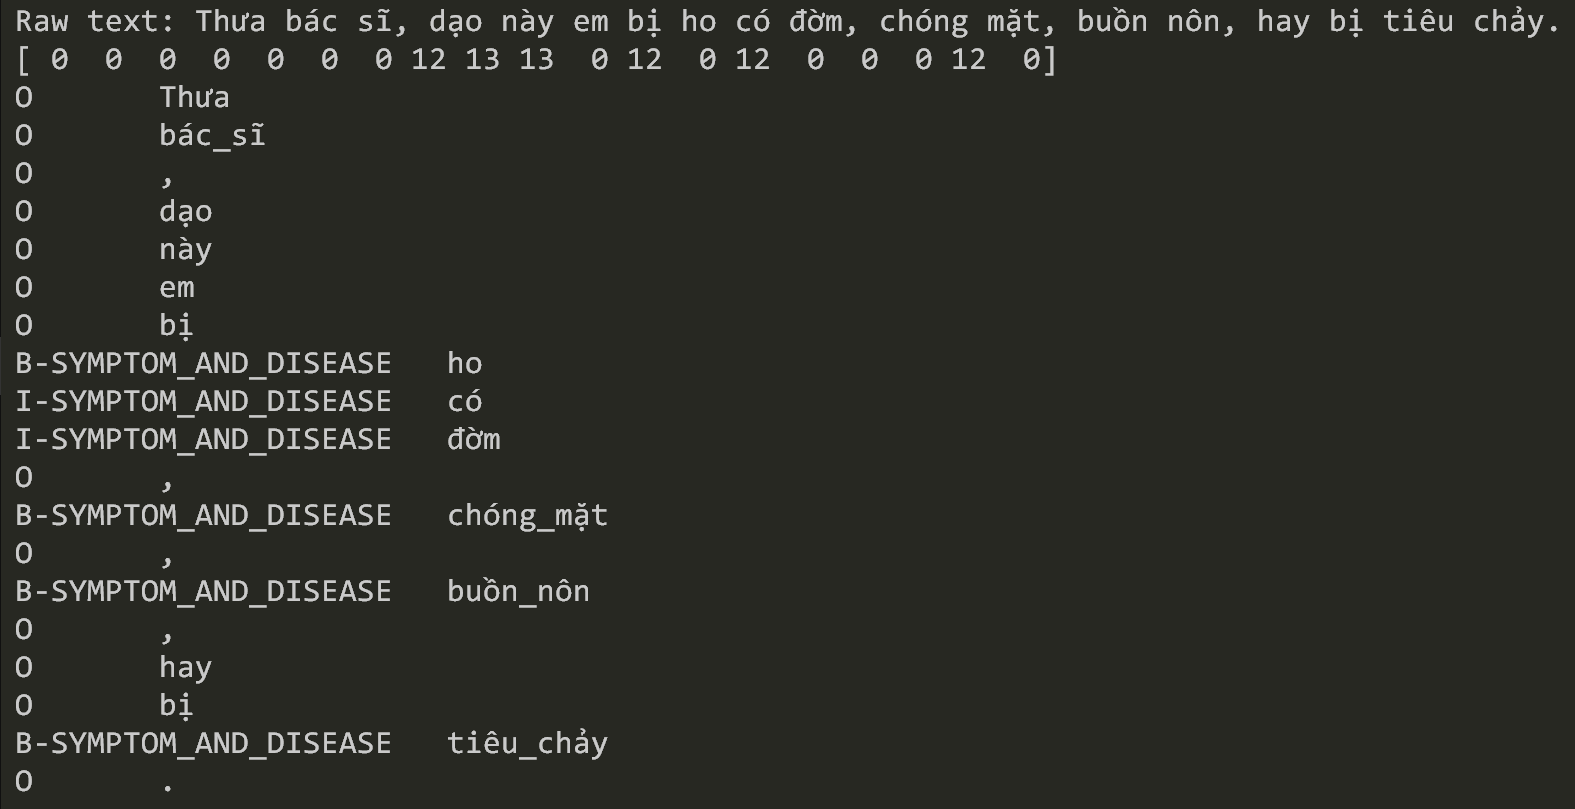
\includegraphics{img/example-result.png}
}
\caption{Một ví dụ cho input (câu văn miêu tả triệu chứng) và output (danh sách các nhãn của câu)}
\label{fig:example-result}
\end{figure}

\begin{figure}[H]
\centering
\resizebox{\textwidth}{!}{
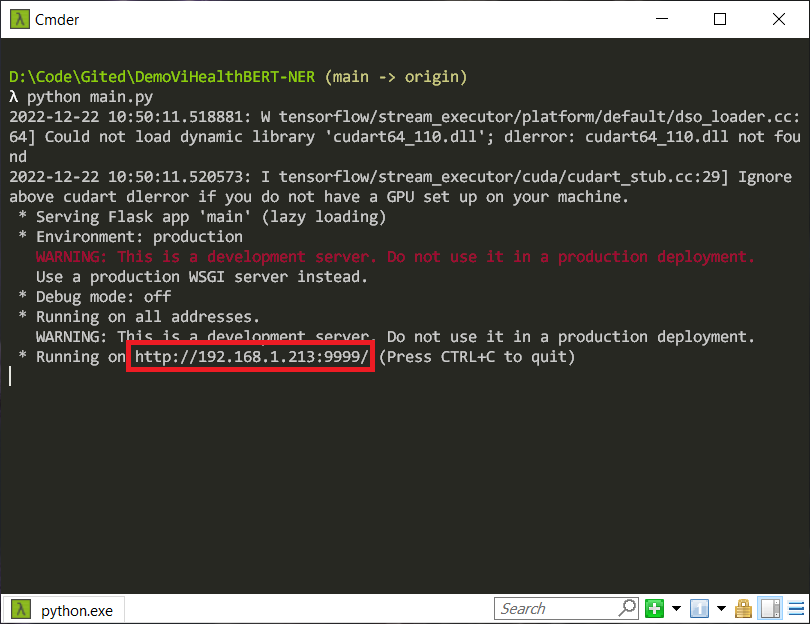
\includegraphics{img/runserver.PNG}
}
\caption{Địa chỉ IP của server sẽ được in ra màn hình terminal lúc khởi động thành công.}
\label{fig:runserver}
\end{figure}

\begin{figure}[H]
\centering
\resizebox{\textwidth}{!}{
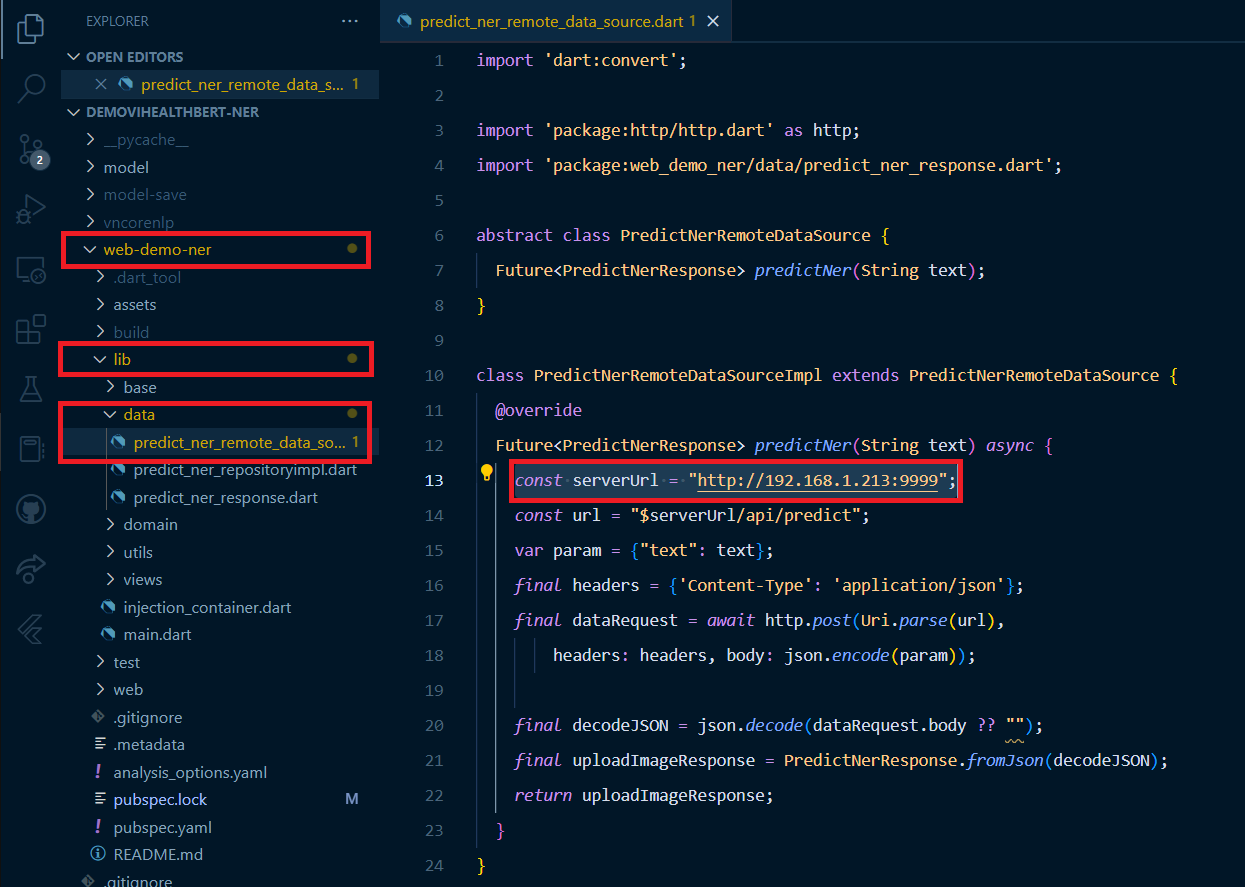
\includegraphics{img/update-frontend.PNG}
}
\caption{Chỉnh sửa IP server cho frontend.}
\label{fig:update-frontend}
\end{figure}

\begin{figure}[H]
\centering
\resizebox{\textwidth}{!}{
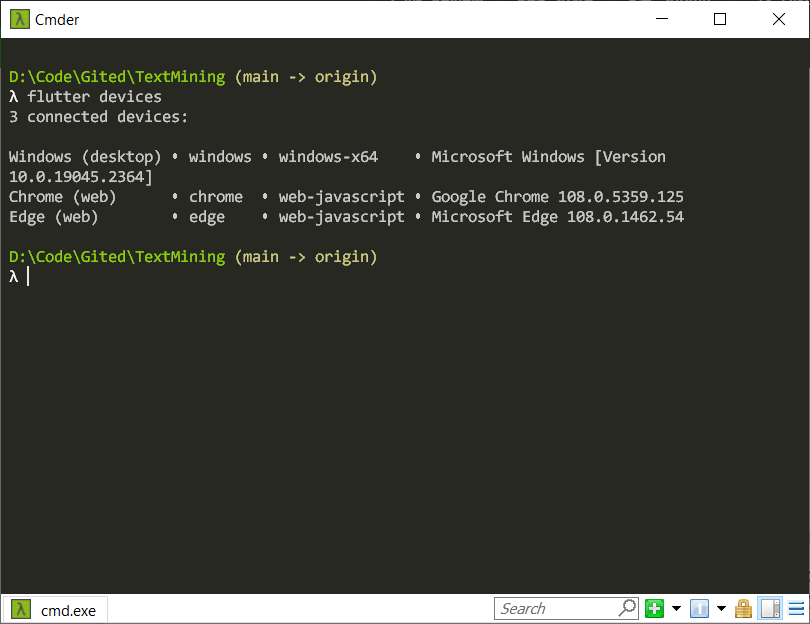
\includegraphics{img/devices.PNG}
}
\caption{Danh sách các devices có thể sử dụng để chạy ứng dụng}
\label{fig:flutter-devices}
\end{figure}

\begin{figure}[H]
\centering
\resizebox{\textwidth}{!}{
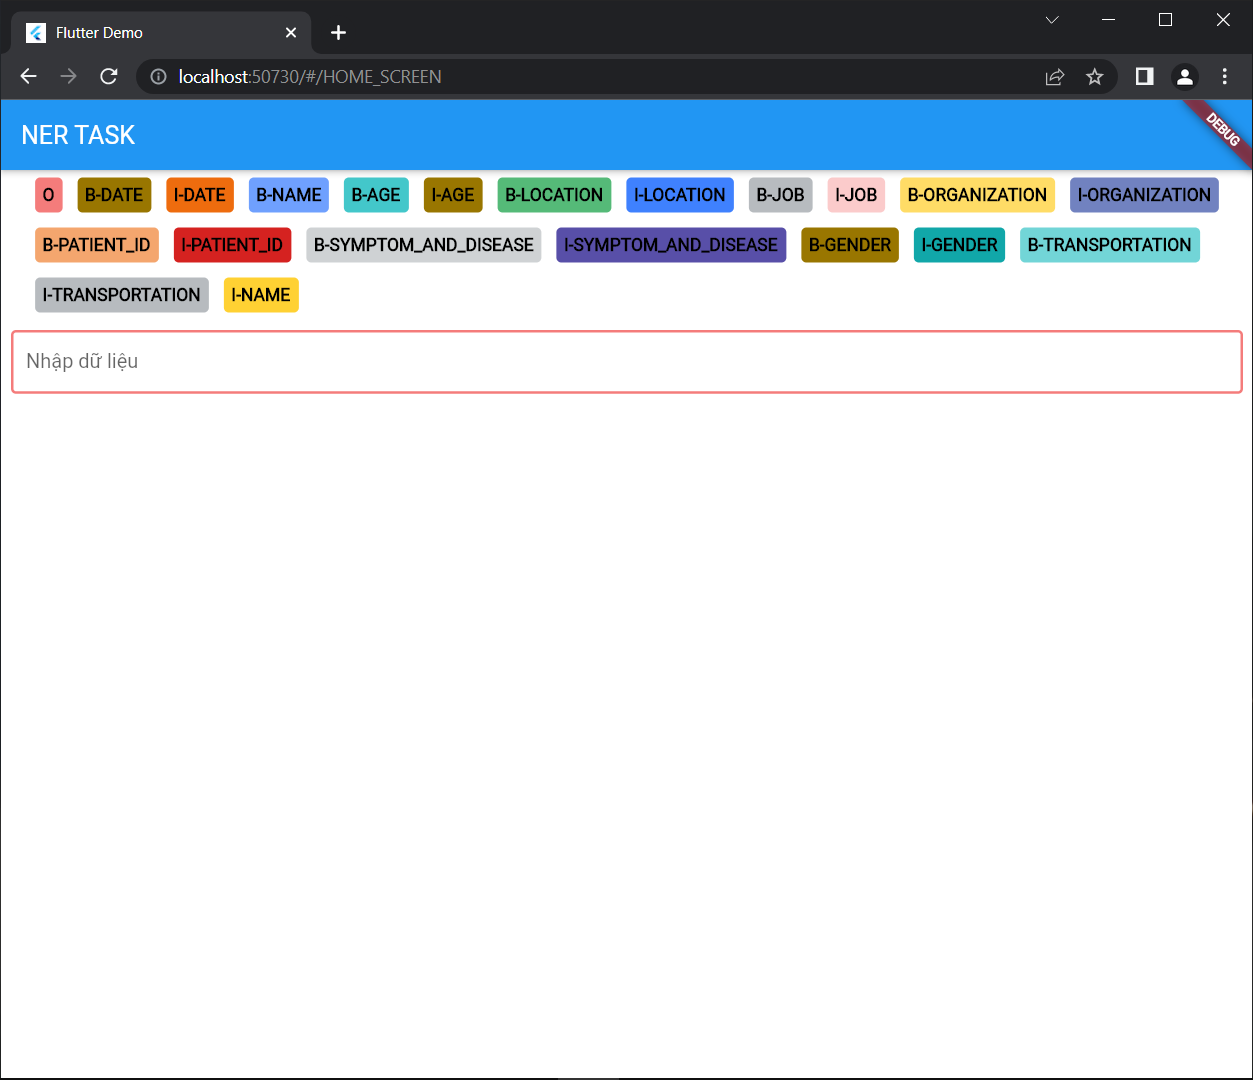
\includegraphics{img/web-demo}
}
\caption{Giao diện ứng dụng trích xuất triệu chứng}
\label{fig:web-demo}
\end{figure}

\begin{figure}[H]
\centering
\resizebox{\textwidth}{!}{
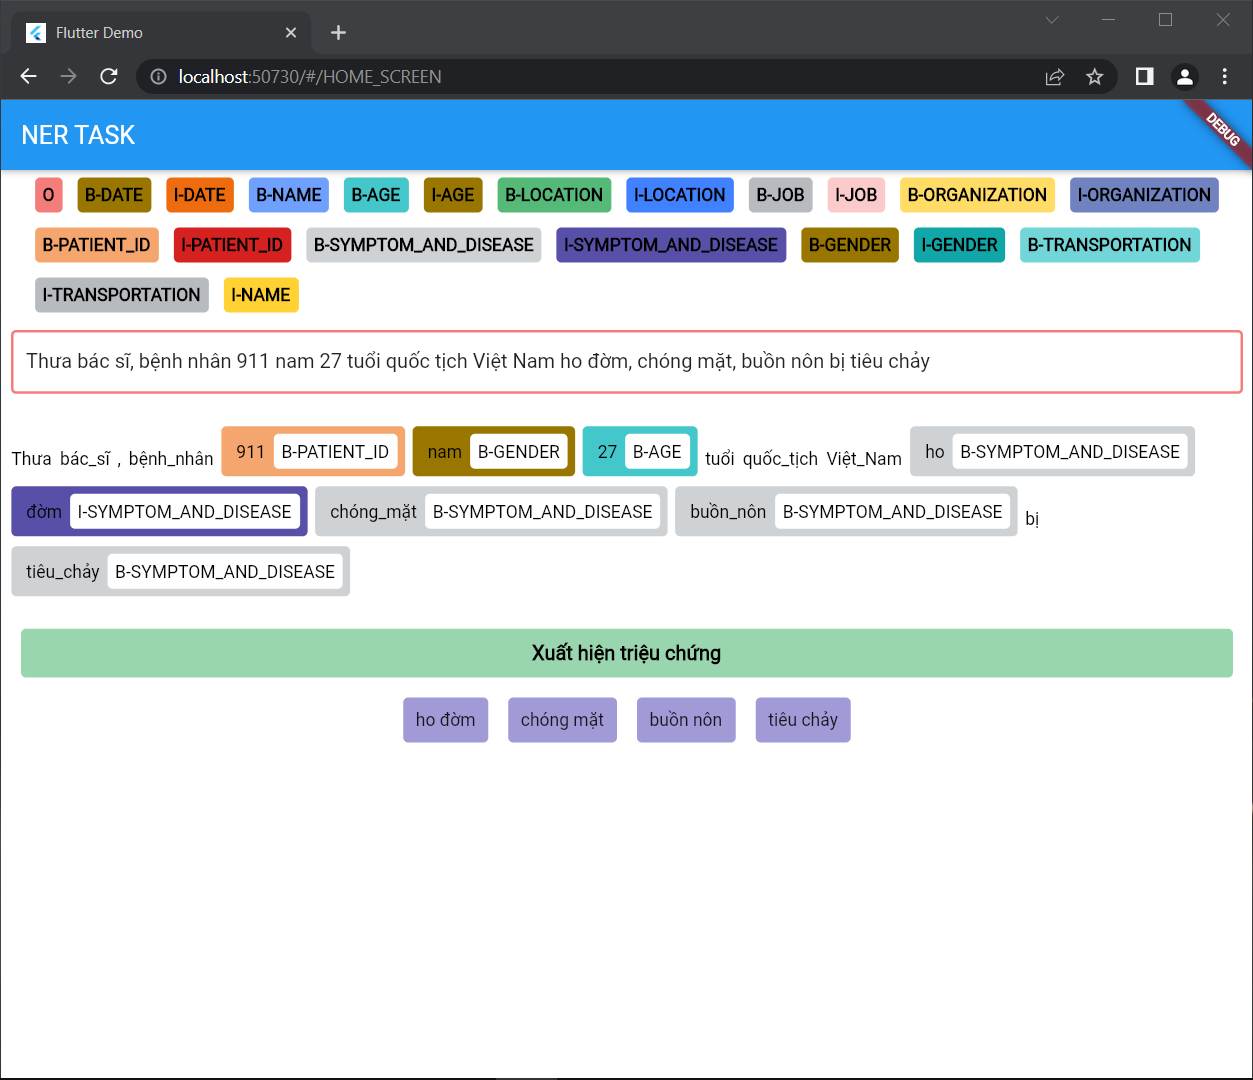
\includegraphics{img/web-demo-result.PNG}
}
\caption{Kết quả trích xuất triệu chứng từ đầu vào của người dùng}
\label{fig:web-demo-result}
\end{figure}
